\begin{figure}[H]
\centering

% --- Row 1 ---------------------------------------------------
\subfloat[Directed SoTS]{%
    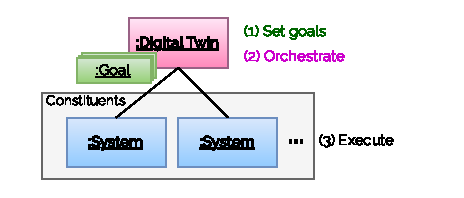
\includegraphics[trim={0.66cm 0.25cm 1.1cm 0.25cm},clip,
    width=0.4\linewidth]{figures/Literature Review/framework/instances/directed.pdf}}
\hfill
\subfloat[Acknowledged SoTS]{%
    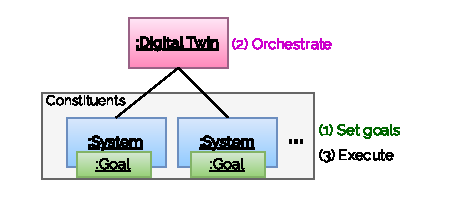
\includegraphics[trim={0.66cm 0.25cm 1.1cm 0.25cm},clip,
    width=0.4\linewidth]{figures/Literature Review/framework/instances/acknowledged.pdf}}
\\[1.2em]

% --- Row 2 ---------------------------------------------------
\subfloat[Collaborative SoTS]{%
    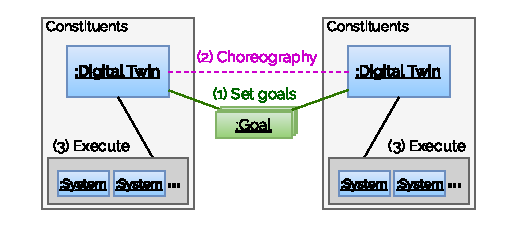
\includegraphics[trim={0.66cm 0.25cm 0.75cm 0.25cm},clip,
    width=0.4\linewidth]{figures/Literature Review/framework/instances/collaborative.pdf}}
\hfill
\subfloat[Virtual SoTS]{%
    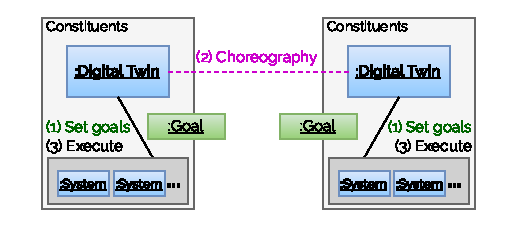
\includegraphics[trim={0.66cm 0.25cm 0.75cm 0.25cm},clip,
    width=0.4\linewidth]{figures/Literature Review/framework/instances/virtual.pdf}}
\\[1.2em]

% --- Row 3 ---------------------------------------------------
\subfloat[System of Specialized DTs]{%
    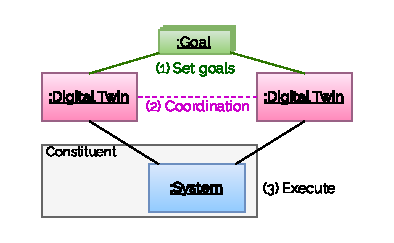
\includegraphics[trim={0.66cm 0.25cm 0.50cm 0.25cm},clip,
    width=0.4\linewidth]{figures/Literature Review/framework/instances/domainspec.pdf}}
\hfill
\subfloat[System of Specialized DTs and Specialized Systems]{%
    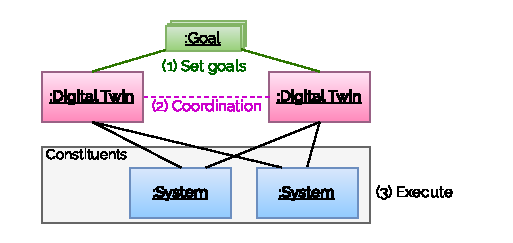
\includegraphics[trim={0.66cm 0.25cm 0.75cm 0.25cm},clip,
    width=0.4\linewidth]{figures/Literature Review/framework/instances/domainspec2.pdf}}

\caption{Overview of the six architectural styles observed in SoTS}
\label{fig:sots-architectures}
\end{figure}
